\section{Build tools: Maven}

\subsection{What is it?}

\begin{flushleft}
\textbf{Maven} is basically a tool that can now be used for building and managing any Java-based project. It addresses two aspects of building software: first, it describes how software is built, and second, it describes its dependencies. By using these two aspects, it can be used for a variety of tasks inside a project, which include building executables, building documentation and downloading dependencies. It is also very extensible, so any features that is doesn't contain normally can be added using plugins. 

\end{flushleft}


\subsection{Objectives}

Maven’s primary goal is to allow a developer to comprehend the complete state of a development effort in the shortest period of time. In order to attain this goal there are several areas of concern that Maven attempts to deal with: 

\begin{enumerate}
\item \textit{Making the build process easy:} provides a lot of shielding from the details.

\item \textit{Providing a uniform build system:} allows a project to build using its project object model (POM) and a set of plugins that are shared by all projects using Maven.

\item \textit{Providing quality project information:} provides plenty of useful project information that is in part taken from your POM and in part generated from your project’s sources (change log,dependency list, unit test).

\item \textit{Providing guidelines for best practices development:} specification, execution, and reporting of unit tests are part of the normal build cycle using Maven.

\item \textit{Allowing transparent migration to new features:} provides an easy way for Maven clients to update their installations so that they can take advantage of any changes that been made to Maven itself.

\end{enumerate}

\subsection{Components}

\begin{itemize}

\item An XML file describes the software project being built, its dependencies on other external modules and components, the build order, directories, and required plug-ins.Please see image \ref{fig:maven}in order to understand the relationship between the components. 

\item It comes with pre-defined targets for performing certain well-defined tasks such as compilation of code and its packaging. 

\item Maven dynamically downloads Java libraries and Maven plug-ins from one or more repositories such as the Maven 2 Central Repository, and stores them in a local cache.This local cache of downloaded artifacts can also be updated with artifacts created by local projects. Public repositories can also be updated.

\end{itemize}



\begin{figure}[h]
    \center{}
    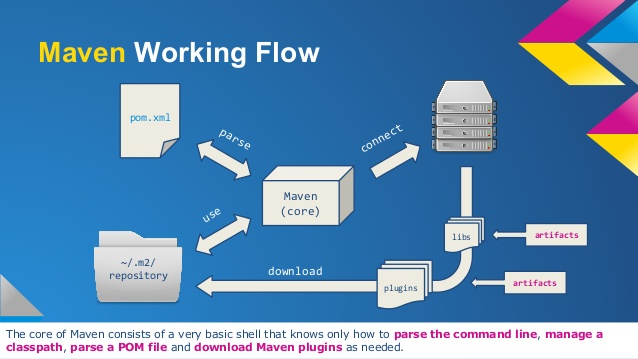
\includegraphics[width=1\textwidth]{maven}
    \caption{Maven Working Flow
    \protect\footnotemark}\label{fig:maven}
\end{figure}
\footnotetext{\url{http://www.slideshare.net/boyw165/note-apache-maven-intro-36821953}}

\subsection{Some Features}

The following are the key features of Maven in a nutshell: 

\begin{itemize}
\item Superior dependency management including automatic updating, dependency closures (also known as transitive dependencies).

\item Able to easily work with multiple projects at the same time.

\item A large and growing repository of libraries and metadata to use out of the box, and arrangements in place with the largest Open Source projects for real-time availability of their latest releases.

\item Extensible, with the ability to easily write plugins in Java or scripting languages.
\item Model based builds: Maven is able to build any number of projects into predefined output types such as a JAR, WAR, or distribution based on metadata about the project, without the need to do any scripting in most cases.

\item Coherent site of project information: Using the same metadata as for the build process, Maven is able to generate a web site or PDF including any documentation you care to add, and adds to that standard reports about the state of development of the project.

\end{itemize}

\subsection{Comparison with Apache Ant}

Please see \textbf{differences} in table \ref{table:differences}

\begin{table}[hb]
    \begin{tabulary}{\textwidth}{cLL}
        \toprule
  \textbf{Aspect} & \textbf{Maven } & \textbf{Apache Ant } \\
        \midrule
  \textbf{Reach } & Covers the whole project build process & Takes care of generating the executable \\
        \midrule
  \textbf{Design} & Uses conventions for the build procedure, and only exceptions need to be written down & All aspects need to be specified \\
        \midrule
  \textbf{Languages Supported} & Can also be used to build and manage projects written in C\#, Ruby, Scala, and other languages&Only used for Java applications \\ 
    \bottomrule
    \end{tabulary}
    \caption{Differences}\label{table:differences}
\end{table}



Please see \textbf{similarities} in table \ref{table:similarities}

\begin{table}[h]
    \begin{tabulary}{\textwidth}{cL}
        \toprule
  \textbf{Aspect} & \textbf{Description} \\
        \midrule
  \textbf{Usage } & Tools that help the developer automate different aspects of a project \\
        \midrule
  \textbf{Technology} & XML Based  \\
        \midrule
  \textbf{Language Support} & Java support \\
    \bottomrule
    \end{tabulary}
    \caption{Similarities}\label{table:similarities}
\end{table}

Sources taken from~\autocites{wiki_maven}{apacheorg_maven}

